%%%%%%%%%%%%%%%%%%% EJERCICIO 10  %%%%%%%

\textbf{Ejemplo 10}\\
¿Cuál es la tasa nominal anual (150 días) vencido equivalente a una tasa del 24\% 
periódica (200 días) anticipada? Asumir el año de 365 días.\\

%\newpage %USAR SOLO SI EL SOLUCIÓN QUEDA SOLO Y ES NECESARIO BAJARLO A LA SIGUIENTE PAGINA
\textbf{Solución }\\
%La tabla ira centrada
\begin{center}
  \renewcommand{\arraystretch}{1.5}% Margenes de las celdas
  %Creación de la cuadricula de 2 columnas
  \begin{longtable}[H]{|C{0.20\linewidth}|C{0.4\linewidth}|C{0.3\linewidth}|}
    %Creamos una linea horizontal
    \hline
    %Definimos el color de la primera fila
    \rowcolor[HTML]{FFB183}
    %%%%% INICIO ASIGNACIÓN PERíODO FOCAL %%%%%%%
    %%%%%%%%%% INICIO TITULO

    %Lo que se hace aquí es mezclar las 3 columnas en una sola
      \multicolumn{3}{|c|}{\cellcolor[HTML]{FFB183}\textbf{1. Asignación período focal}}                                                                                                        \\ \hline
      \multicolumn{3}{|c|}{$pf: \textit{No aplica}$}                                                                                                                                              
      \\ \hline

    %%%%%%%%%% FIN TITULO
    %%%%% INICIO DECLARACIÓN DE VARIABLES %%%%%%%
    %%%%%%%%%% INICIO TITULO
    %Lo que se hace aquí es mezclar las 3 columnas en una sola
    \multicolumn{3}{|c|}{\cellcolor[HTML]{FFB183}\textbf{2. Declaración de variables}}                                                                 \\ \hline
    %%%%%%%%%% FIN TITULO
    %%%%%%%%%% INICIO SUBTITULO
    \cellcolor[HTML]{FFB183}\textbf{Valores monetarios}    & 
    \cellcolor[HTML]{FFB183}\textbf{Valores no monetarios} &
    \cellcolor[HTML]{FFB183}\textbf{Incógnitas}  \\ \hline
    %%%%%%%%%% FIN SUBTITULO
    %%%%%%%%%% INICIO DE MATEMÁTICAS
    %Cada & hace referencia al paso de la siguiente columna
    & $i_{a1}= 24\% \textit{ p(200 días)a}$ & $j_{2} = ?\% \textit{ na(150 días)v}$  \\ 
    & $m_{1} =\frac{365 \textit{ días}}{200 \textit{ días}}= 1,82 \textit{ p(200 días)a}$  & \\
    & $m_{2} = \frac{365 \textit{ días}}{150 \textit{ días}} = 2,43 \textit{ p(150 días)v}$ &    \\ \hline
    
    %%%%%%%%%% FIN DE MATEMÁTICAS
    %%%%% FIN DECLARACIÓN DE VARIABLES

    %%%%% INICIO FLUJO DE CAJA
    \rowcolor[HTML]{FFB183}
    \multicolumn{3}{|c|}{\cellcolor[HTML]{FFB183}\textbf{3. Diagrama de equivalencia de tasas}}                                                        \\ \hline
    %Mezclamos 3 columnas y pondremos el dibujo
    %%%%%%%%%%%%% INSERCIÓN DE LA IMAGEN
    %Deberán descargar las imágenes respectivas del drive y pegarlas en la carpeta
    %n_capitulo/img/ejemplos/1/capitulo1ejemplo1.pdf  (el /1/ es el numero del ejemplo)

    \multicolumn{3}{|c|}{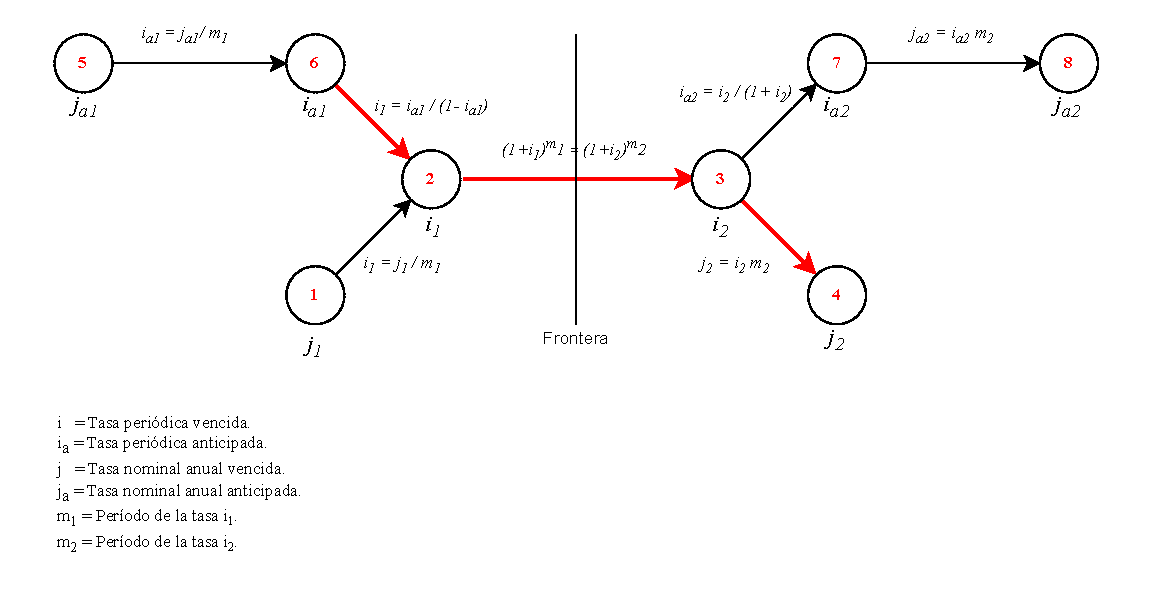
\includegraphics[height = 7.0 cm]{2_Capitulo/ejemplos/10/Capitulo2Ejercicio10.pdf}} \\ \hline
    
    %%%%%%%%%%%%% FIN INSERCIÓN DE IMAGEN
    %%%%%FIN FLUJO DE CAJA

    %%%%% INICIO DECLARACIÓN FORMULAS
    %%%%%%%%%%% INICIO TITULO
    \rowcolor[HTML]{FFB183}
    \multicolumn{3}{|c|}{\cellcolor[HTML]{FFB183}\textbf{4. Declaración de fórmulas}}                                                                  \\ \hline
    %%%%%%%%%%% FIN TITULO
    %%%%%%%%%%% INICIO MATEMÁTICAS

    \multicolumn{3}{|c|}{$i_{1} = \frac{i_{1}}{1-{i_{a1}}} \hspace{0.3cm} \textit{ Tasa periódica vencida }$}  \\
    \multicolumn{3}{|c|}{$j=i(m)\hspace{0.3cm} \textit{Tasa periódica anualizada}$} \\
    \multicolumn{3}{|c|}{$(1+i_{1})^{m_{1}}=(1+i_{2})^{m_{2}} \hspace{0.3cm} \textit{ Equivalencia de tasas}$ } \\ \hline
    %%%%%%%%%% FIN MATEMÁTICAS
    %%%%%% INICIO DESARROLLO MATEMÁTICO
    \rowcolor[HTML]{FFB183}
    %%%%%%%%%%INICIO TITULO
    \multicolumn{3}{|c|}{\cellcolor[HTML]{FFB183}\textbf{5. Desarrollo matemático}}                                                                    \\ \hline
    %%%%%%%%%% FIN TITULO
    %%%%%%%%%% INICIO MATEMÁTICAS
    \multicolumn{3}{|c|}{$i_{1} = \frac{0.24}{1-0,24} = 0,3158 \textit{p(200 días)v}$} \\
    \multicolumn{3}{|c|}{$(1 + 0,3158)^{1,82}= (1 + i_{2})^{2,43} $} \\
    \multicolumn{3}{|c|}{$(1,3158)^{\frac{1,82}{2,43}}-1=i_{2}$} \\
    \multicolumn{3}{|c|}{$i_{2}=0,2282 \textit{ p(150 días)v} \equiv 22,82\% \textit{ p(150 días)v}$} \\ 
    \multicolumn{3}{|c|}{$j_{2}=22,82\% (2,43)$} \\
    \multicolumn{3}{|c|}{\textit{$j_{2} = 55,45\% \textit{ na(150 días)v}$}} \\ \hline
    %%%%%%%%%% FIN MATEMÁTICAS
    %%%%%% FIN DESARROLLO MATEMÁTICO
    %%%%%% INICIO RESPUESTA
    \rowcolor[HTML]{FFB183}
    %%%%%%%%%%INICIO TITULO
    \multicolumn{3}{|c|}{\cellcolor[HTML]{FFB183}\textbf{6. Respuesta}}                                                                                \\ \hline
    %%%%%%%%%% FIN TITULO
    %%%%%%%%%% INICIO RESPUESTA MATEMÁTICA
    \multicolumn{3}{|c|}{$j_{2} = 55,45\% \textit{ na(150 días)v}$} \\ \hline
    %%%%%%%%%% FIN MATEMÁTICAS
    %%%%%% FIN RESPUESTA
  \end{longtable}
  %Se crean dos lineas en blanco para que no quede el siguiente texto tan pegado
  %\newline \newline %USARLO SI CREES QUE ES NECESARIO
\end{center}
%%%%%%%%%%%%%%%%%%% FIN EJERCICIO 10  %%%%%%%%%%%%%%%%%%%%%%%%%%%%%%
